\section{Models}
\label{sec:models}

\subsection{Shared-encoder Gaussian residual prediction}
\label{sec:notation}
\label{sec:s1}

A training example contains an observed input $x$, a target $y$, and an auxiliary observation $u$ that is available only during training. MPI3D also supplies a command $a$; we omit it on Moving-MNIST. An encoder $f$, comprising a backbone and projector, maps observations to 128-dimensional embeddings. The predictor $g$ takes the source embedding $z_x=f(x)$, the command if present, and a residual $r$: a low-dimensional random variable intended to carry the part of the outcome that the source does not determine. A diagonal Gaussian prior $p_\theta(r\mid z_x,a)$ sees only the observed information; a diagonal Gaussian posterior $q_\phi(r\mid z_x,a,z_u)$ also sees $z_u=f(u)$. On Moving-MNIST, $u$ is a later clip of the same trajectory; on MPI3D, $u=y$ (Section~\ref{sec:posterior-inputs}). The residual has two coordinates on Moving-MNIST and one on MPI3D.

\shvar{} uses the same encoder for source and target, $z_y=f(y)$, and trains with
\begin{equation}
\label{eq:s1}
\begin{aligned}
\mathcal L ={}& -\frac1B\sum_{b=1}^{B}\cos\!\big(g(z_{x,b},a_b,r_b),z_{y,b}\big)\\
&+\frac{\beta}{B}\sum_{b=1}^{B}\mathrm{KL}\!\big(q_\phi(r\mid z_{x,b},a_b,z_{u,b})\,\big\|\,p_\theta(r\mid z_{x,b},a_b)\big)\\
&+\frac{\lambda}{2}\big[\mathrm{SIGReg}(\{z_{x,b}\}_b)+\mathrm{SIGReg}(\{z_{y,b}\}_b)\big],
\end{aligned}
\end{equation}
where $r_b$ is a reparameterized posterior draw~\citep{kingma2014vae}, $\beta=0.001$ and $\lambda=0.1$. We denote the three unweighted losses by $\mathcal L_{\mathrm{pred}}$, $\mathcal L_{\mathrm{KL}}$ and $\mathcal L_{\mathrm{SIG}}$. The latent prediction term aligns predictions with the model's own target embeddings. The KL term matches the posterior to the learned prior. SIGReg regularizes the real source and target projector outputs toward an isotropic Gaussian~\citep{balestriero2025lejepa,maes2026lewm}. It is applied before cosine normalization, and not to predictions or to the separate Moving-MNIST posterior clip. Source, target and posterior-feature gradients all reach the one encoder. Appendix~\ref{app:arch} gives the Gaussian heads, objective reductions and SIGReg estimator.

\subsection{Four-model comparison}
\label{sec:roles}

\begin{table}[t]
\caption{Training recipes crossed with prediction families: deterministic (Det) or Gaussian residual (Var). All models use $\mathcal L_{\mathrm{pred}}$ plus the listed losses, with $\beta=0.001$ and $\lambda=0.1$ where applicable. Parentheses count stored encoders. EMA momentum is 0.996 on Moving-MNIST and increases from 0.996 to 1 on MPI3D. Appendix~\ref{app:modeldetails} specifies target gradients and batch-normalization updates.}
\label{tab:roles}
\centering
\small
\setlength{\tabcolsep}{4pt}
\begin{tabular}{@{}llll@{}}
\toprule
Model & Target branch (encoders) & Residual $r$ & Additional losses \\
\midrule
\emadet{} & EMA, stopped (2) & none & -- \\
\emavar{} & EMA, stopped (2) & Gaussian & $\beta\mathcal{L}_{\mathrm{KL}}$ \\
\shdet{} & Shared, gradients (1) & none & $\lambda\mathcal{L}_{\mathrm{SIG}}$ \\
\shvar{} & Shared, gradients (1) & Gaussian & $\beta\mathcal{L}_{\mathrm{KL}}+\lambda\mathcal{L}_{\mathrm{SIG}}$ \\
\bottomrule
\end{tabular}

\end{table}

\begin{figure}[t]
\centering
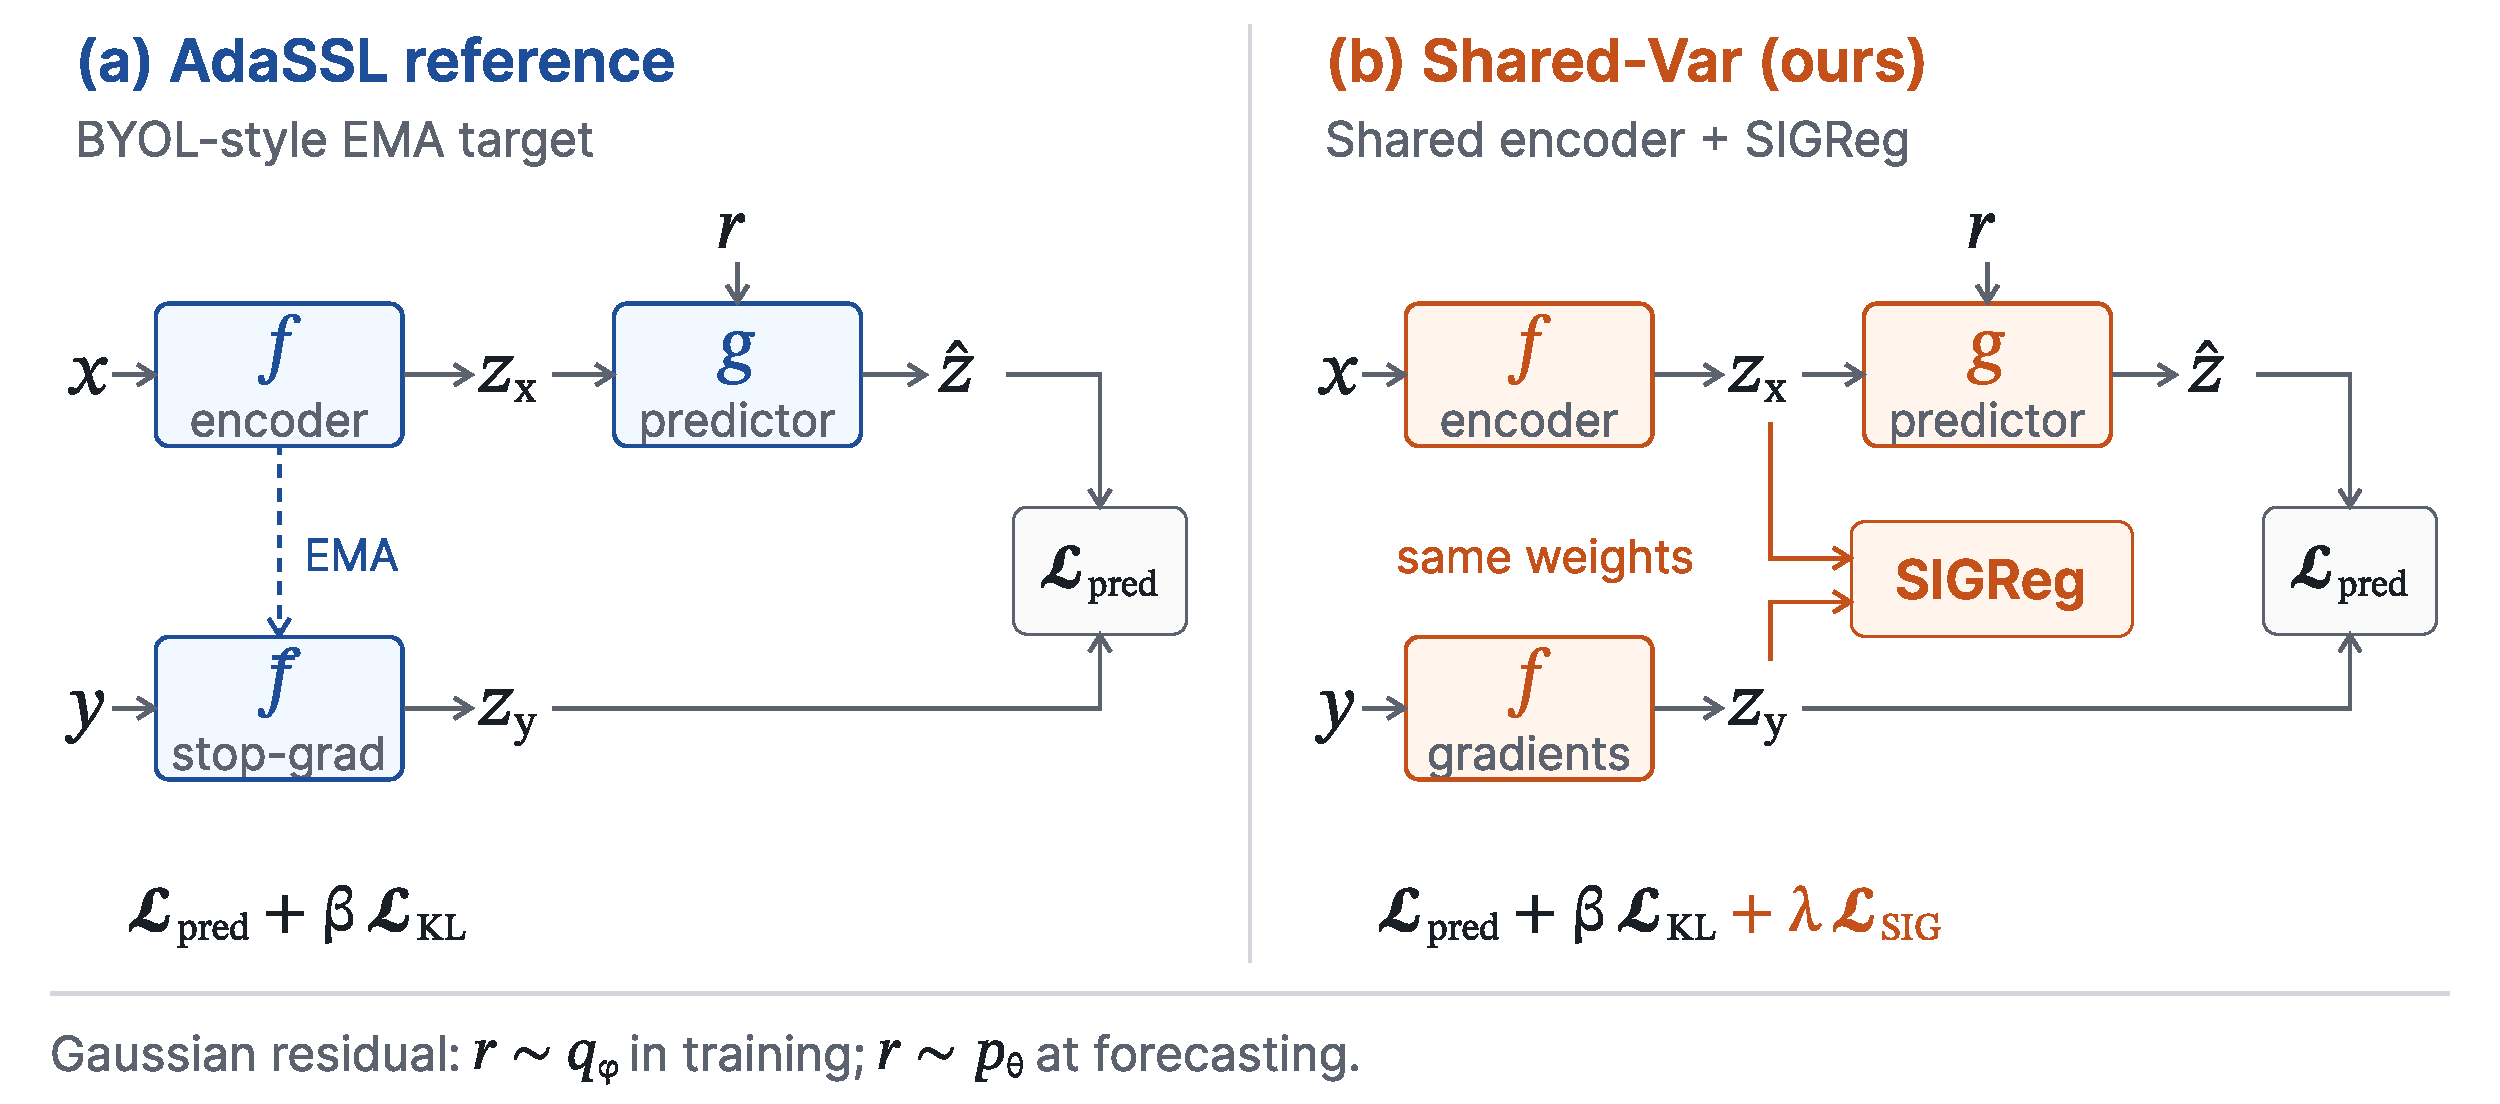
\includegraphics[width=\linewidth]{figures/model_information_flow.pdf}
\caption{Training paths of the two variational models. (a) The \emavar{} uses a BYOL-style EMA target $\bar f$ with stopped target gradients. (b) \shvar{} shares $f$ across source and target, propagates target gradients and adds SIGReg on $z_x$ and $z_y$. Both use the Gaussian residual $r$ and the posterior--prior KL term. For clarity, the posterior and its input $u$, the MPI3D command and the evaluation readout are not drawn; Appendix Algorithm~\ref{alg:train} gives the complete update.}
\label{fig:flow}
\end{figure}

Our two EMA references are the \emadet{} (deterministic) and the \emavar{} (Gaussian residual), local adaptations of BYOL~\citep{grill2020byol} and AdaSSL's video recipe~\citep{zhang2026adassl} to our prediction tasks. Both use an online encoder $f$ and a stopped target $z_y=\mathrm{sg}[\bar f(y)]$, where $\bar f$ is an EMA copy of $f$. The \emavar{} adds the Gaussian residual to the \emadet{}; its posterior consumes differentiable online features, while the alignment target stays stopped. The Shared models use $z_y=f(y)$ with gradients through both views and add SIGReg; \shvar{} adds the Gaussian residual to \shdet{}. Table~\ref{tab:roles} lists the four objectives, and Figure~\ref{fig:flow} contrasts the two variational models.

Relative to the \emavar{}, \shvar{} removes the EMA encoder, its momentum update and its separate batch-normalization (BN) statistics. It adds SIGReg, its coefficient and fixed estimator settings. We use the same $\beta$ as the \emavar{} and the same $\lambda$ as \shdet{}, without tuning either for \shvar{}. The EMA/Shared contrast changes target gradients, regularization and BN exposure together, and adding the residual also adds heads and training information. The design therefore compares whole recipes rather than isolating individual mechanisms.

\subsection{Posterior information and forecasting}
\label{sec:posterior-inputs}
\label{sec:inference}

On Moving-MNIST, the source is frames 1--3, the target is frames 4--6, and the posterior observes frames 7--9 of the same trajectory. The velocity changes once, between frames 3 and 4, and then stays constant (Section~\ref{sec:data-mm}), so the later clip reveals the realized change without being the alignment target. On MPI3D the posterior observes the realized target image: the \emavar{} encodes it through an extra online pass, while \shvar{} reuses $z_y$.

At inference, the variational models encode only the source (and command) and sample the residual from the learned prior; neither the posterior nor $u$ is used. The deterministic models produce one embedding. Each model's fitted readout maps predicted embeddings to velocity or position (Section~\ref{sec:evaluation}). Because the predictor is nonlinear, the forecast distribution need not be Gaussian even though the residual is. Appendix Algorithms~\ref{alg:train} and~\ref{alg:infer} give one training update and one forecast. Eq.~\eqref{eq:s1} is a latent prediction objective; we derive no image-likelihood bound for it.
